\appendix
\renewcommand{\thesection}{APPENDIX \Alph{section}}
\section{ - Figures} \label{appendix:A}
\topskip0pt
\vspace*{\fill}
\begin{center}
    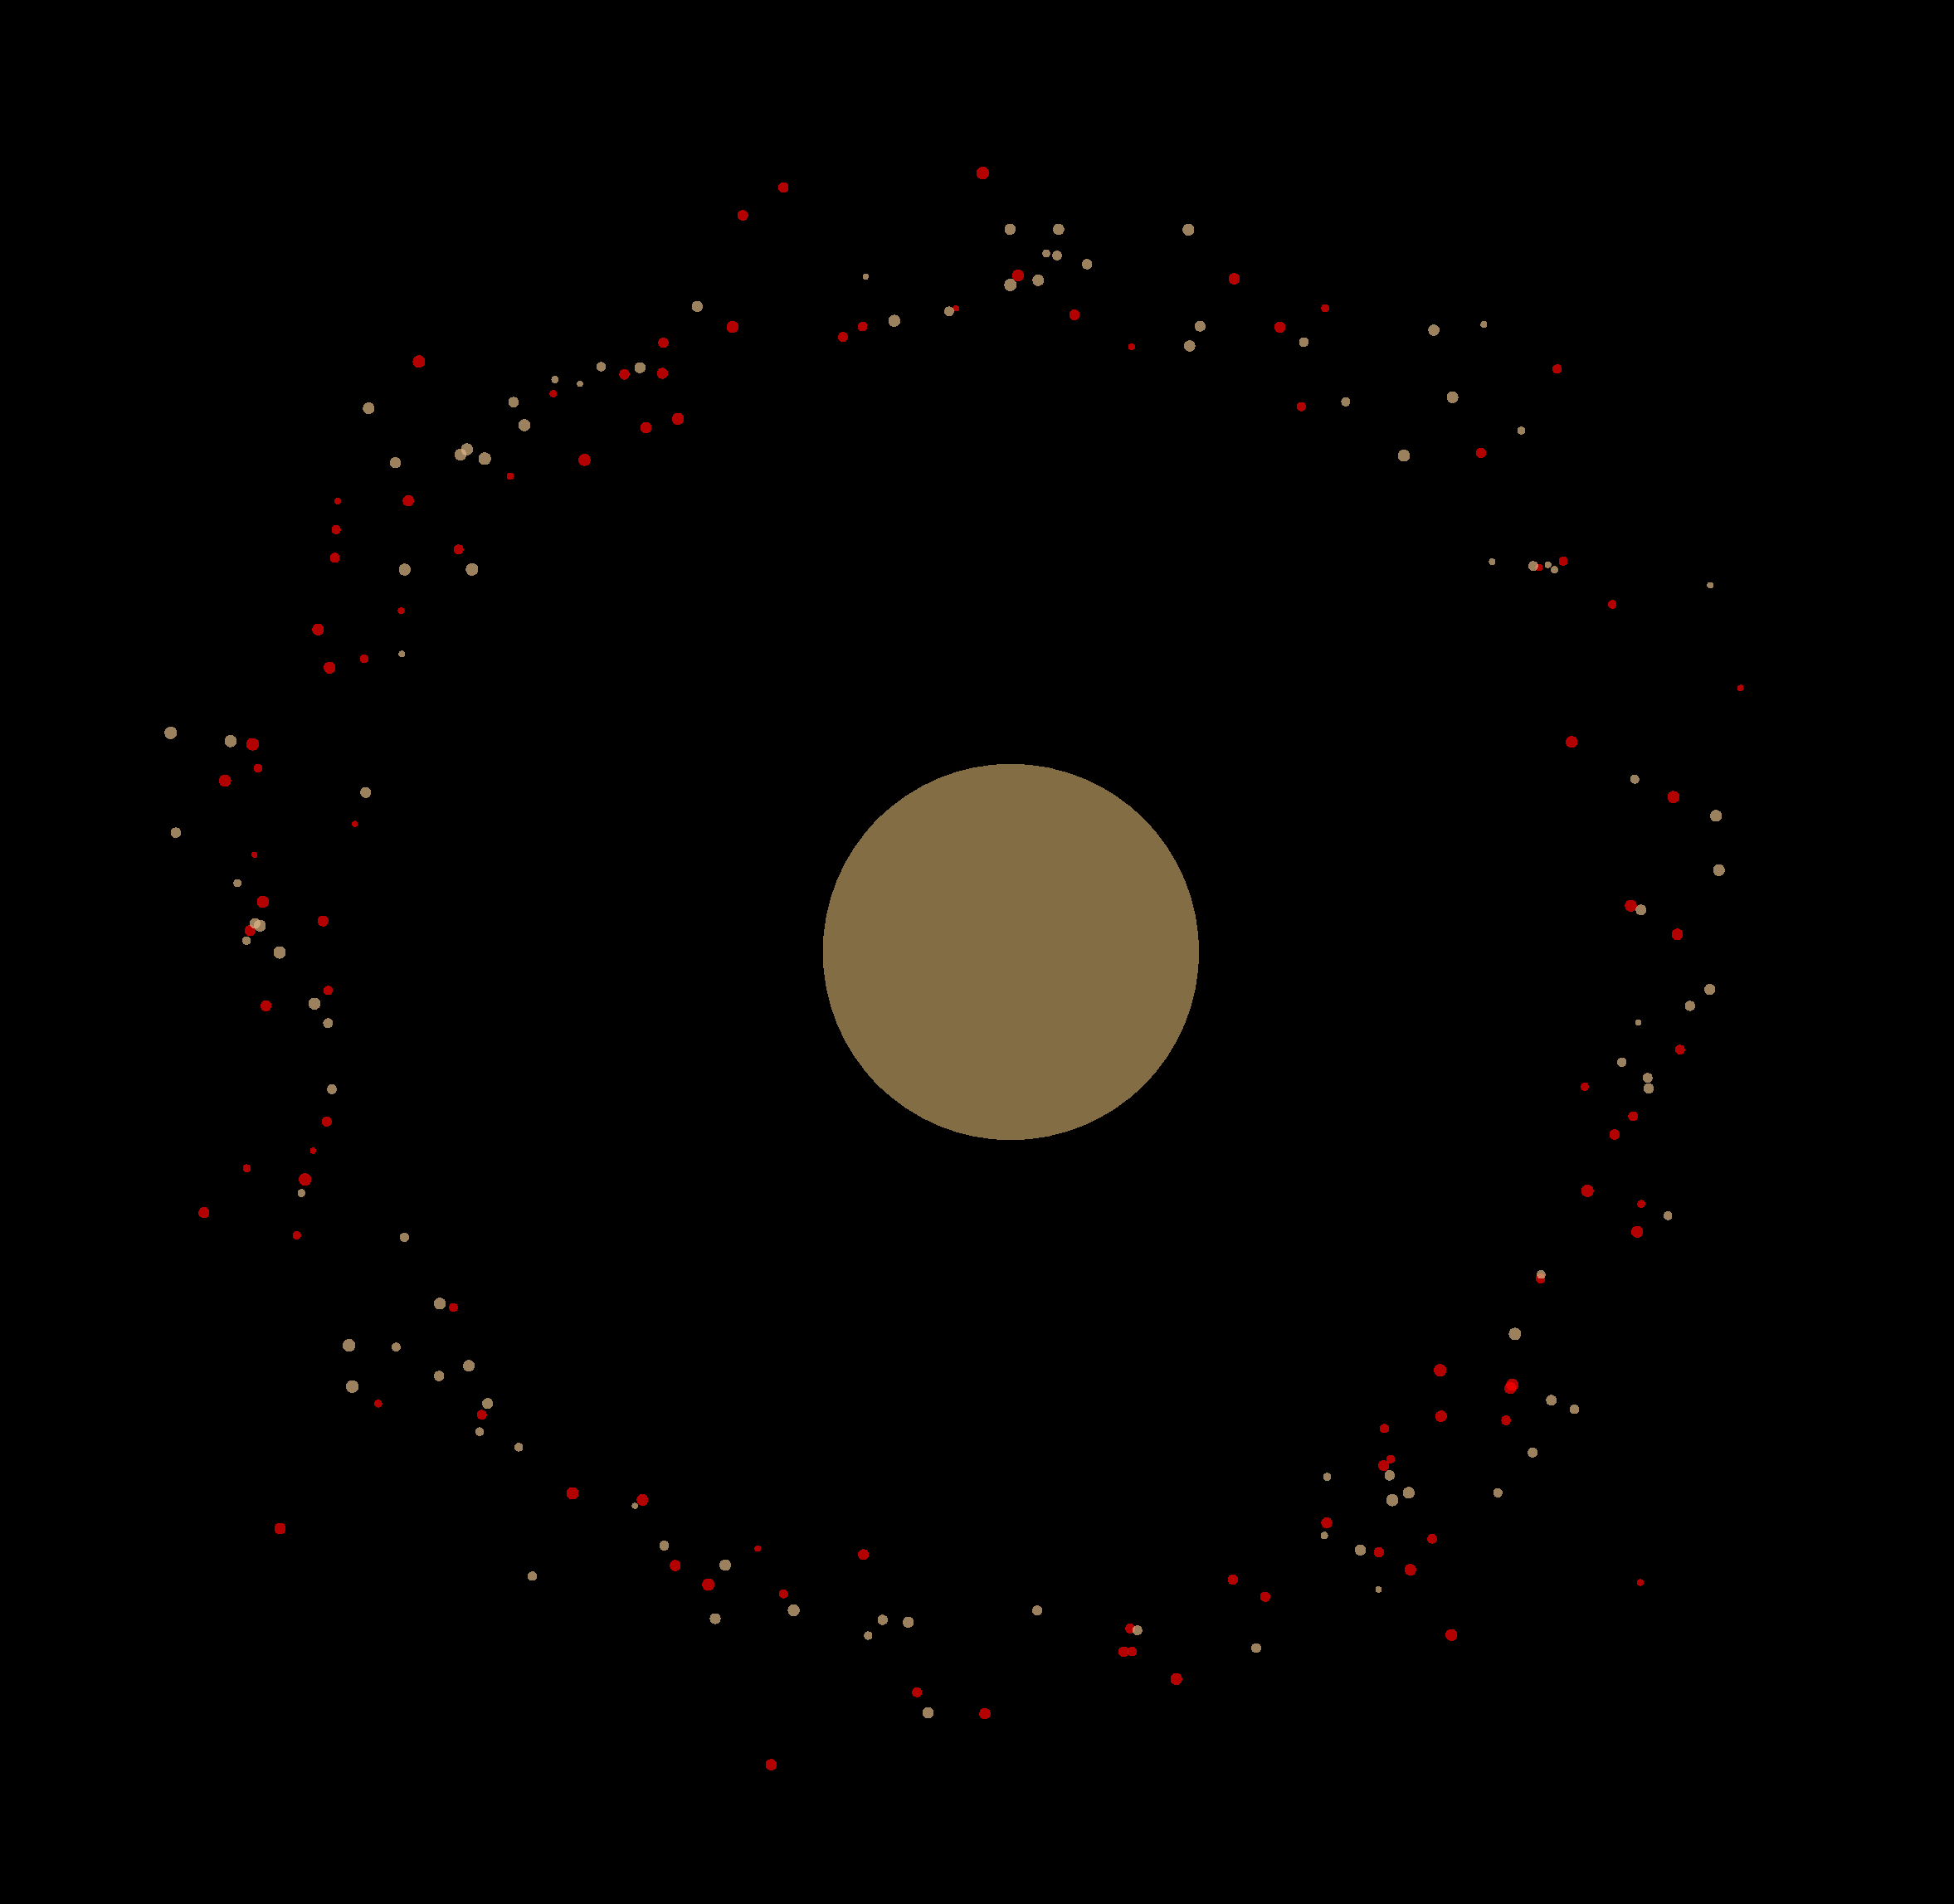
\includegraphics[width=\textwidth]{{img_src/scatter_final_max_5_y_dt_0.001_y}.pdf}
    \captionof{figure}{The starting and final positions of the asteroids with $dt = 0.001$ years and $t_max = 5$ years. The red dots indicates the final positions, while the burly wood colored points are the starting locations.} \label{fig:2}
\end{center}
\vspace*{\fill}
\newpage
\topskip0pt
\vspace*{\fill}
\begin{center}
    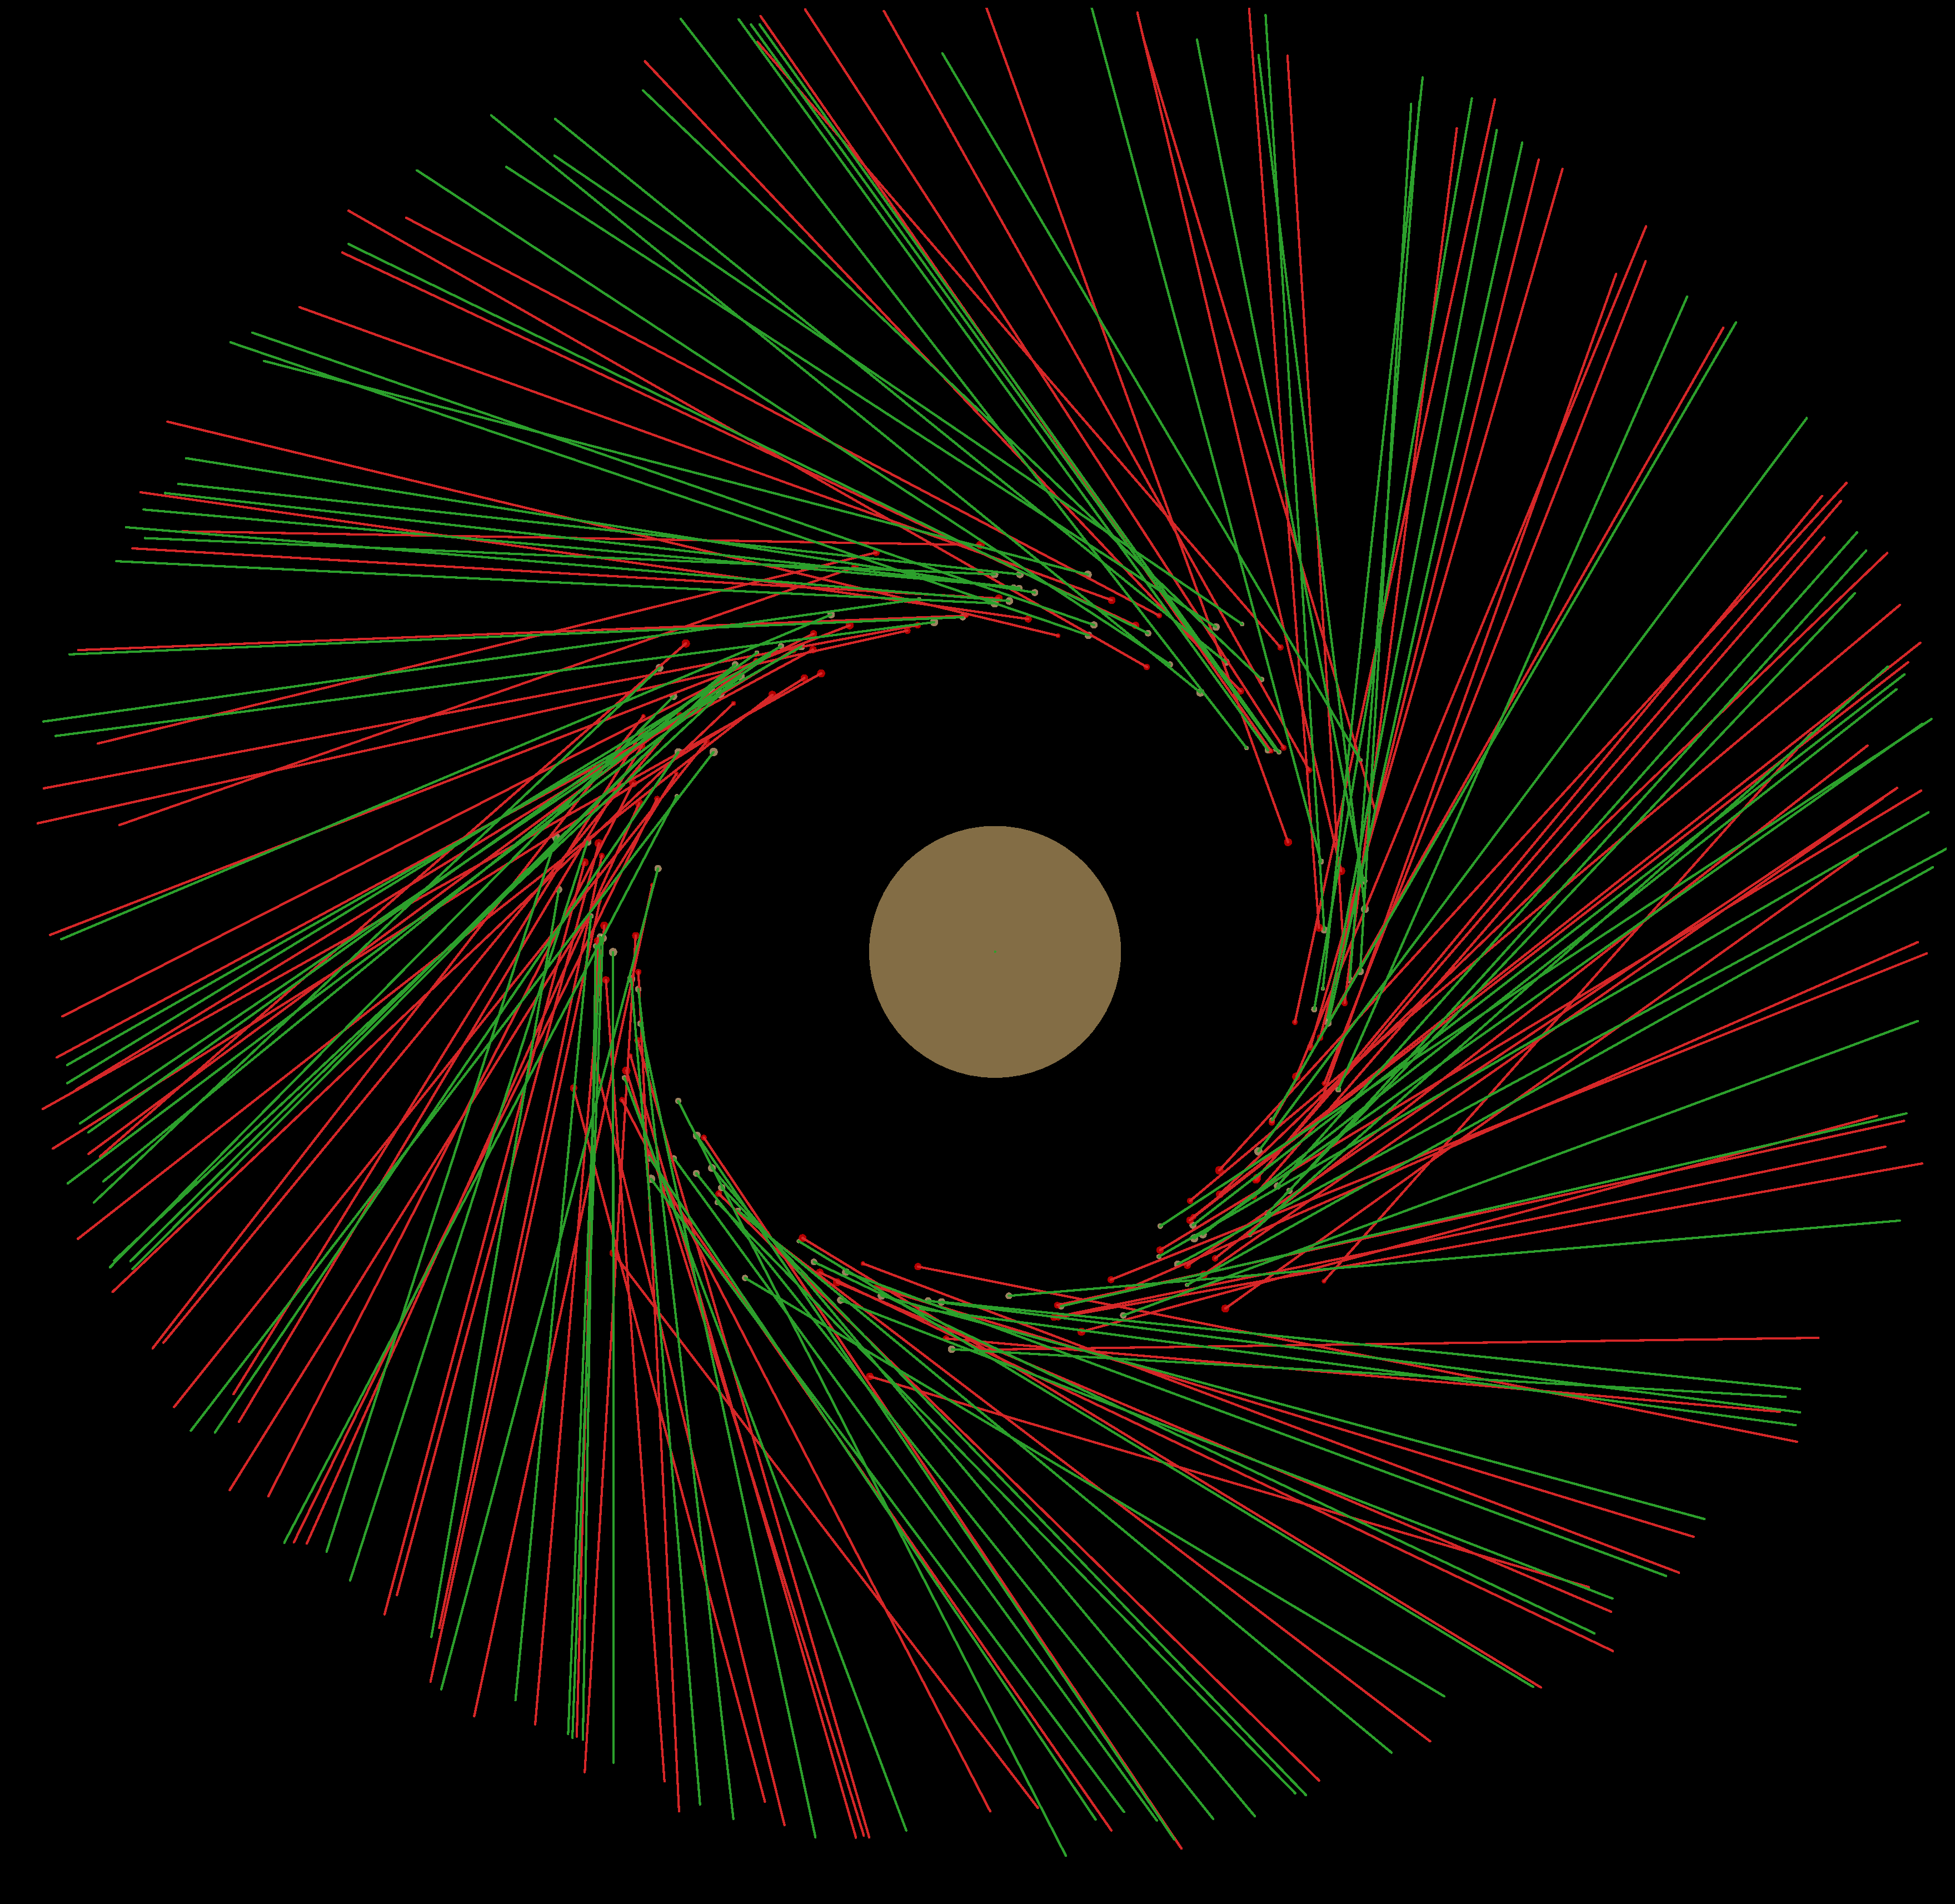
\includegraphics[width=\textwidth]{{img_src/velocity_final_max_5_y_dt_0.001_y}.pdf}
    \captionof{figure}{The starting and final positions and corresponding velocity vectors of the asteroids with $dt = 0.001$ years and $t_max = 5$ years. The red dots with red lines indicates the final positions and velocities, while the burly wood colored points and green lines are the starting locations and velocities.} \label{fig:3}
\end{center}
\vspace*{\fill}